\chapter{3D Vision}

\section{Image Formation}

The basic model is based on the principle of \textbf{camera obscura}, a room with a hole by which the light can enter the room.

\begin{figure}[H]
    \centering
    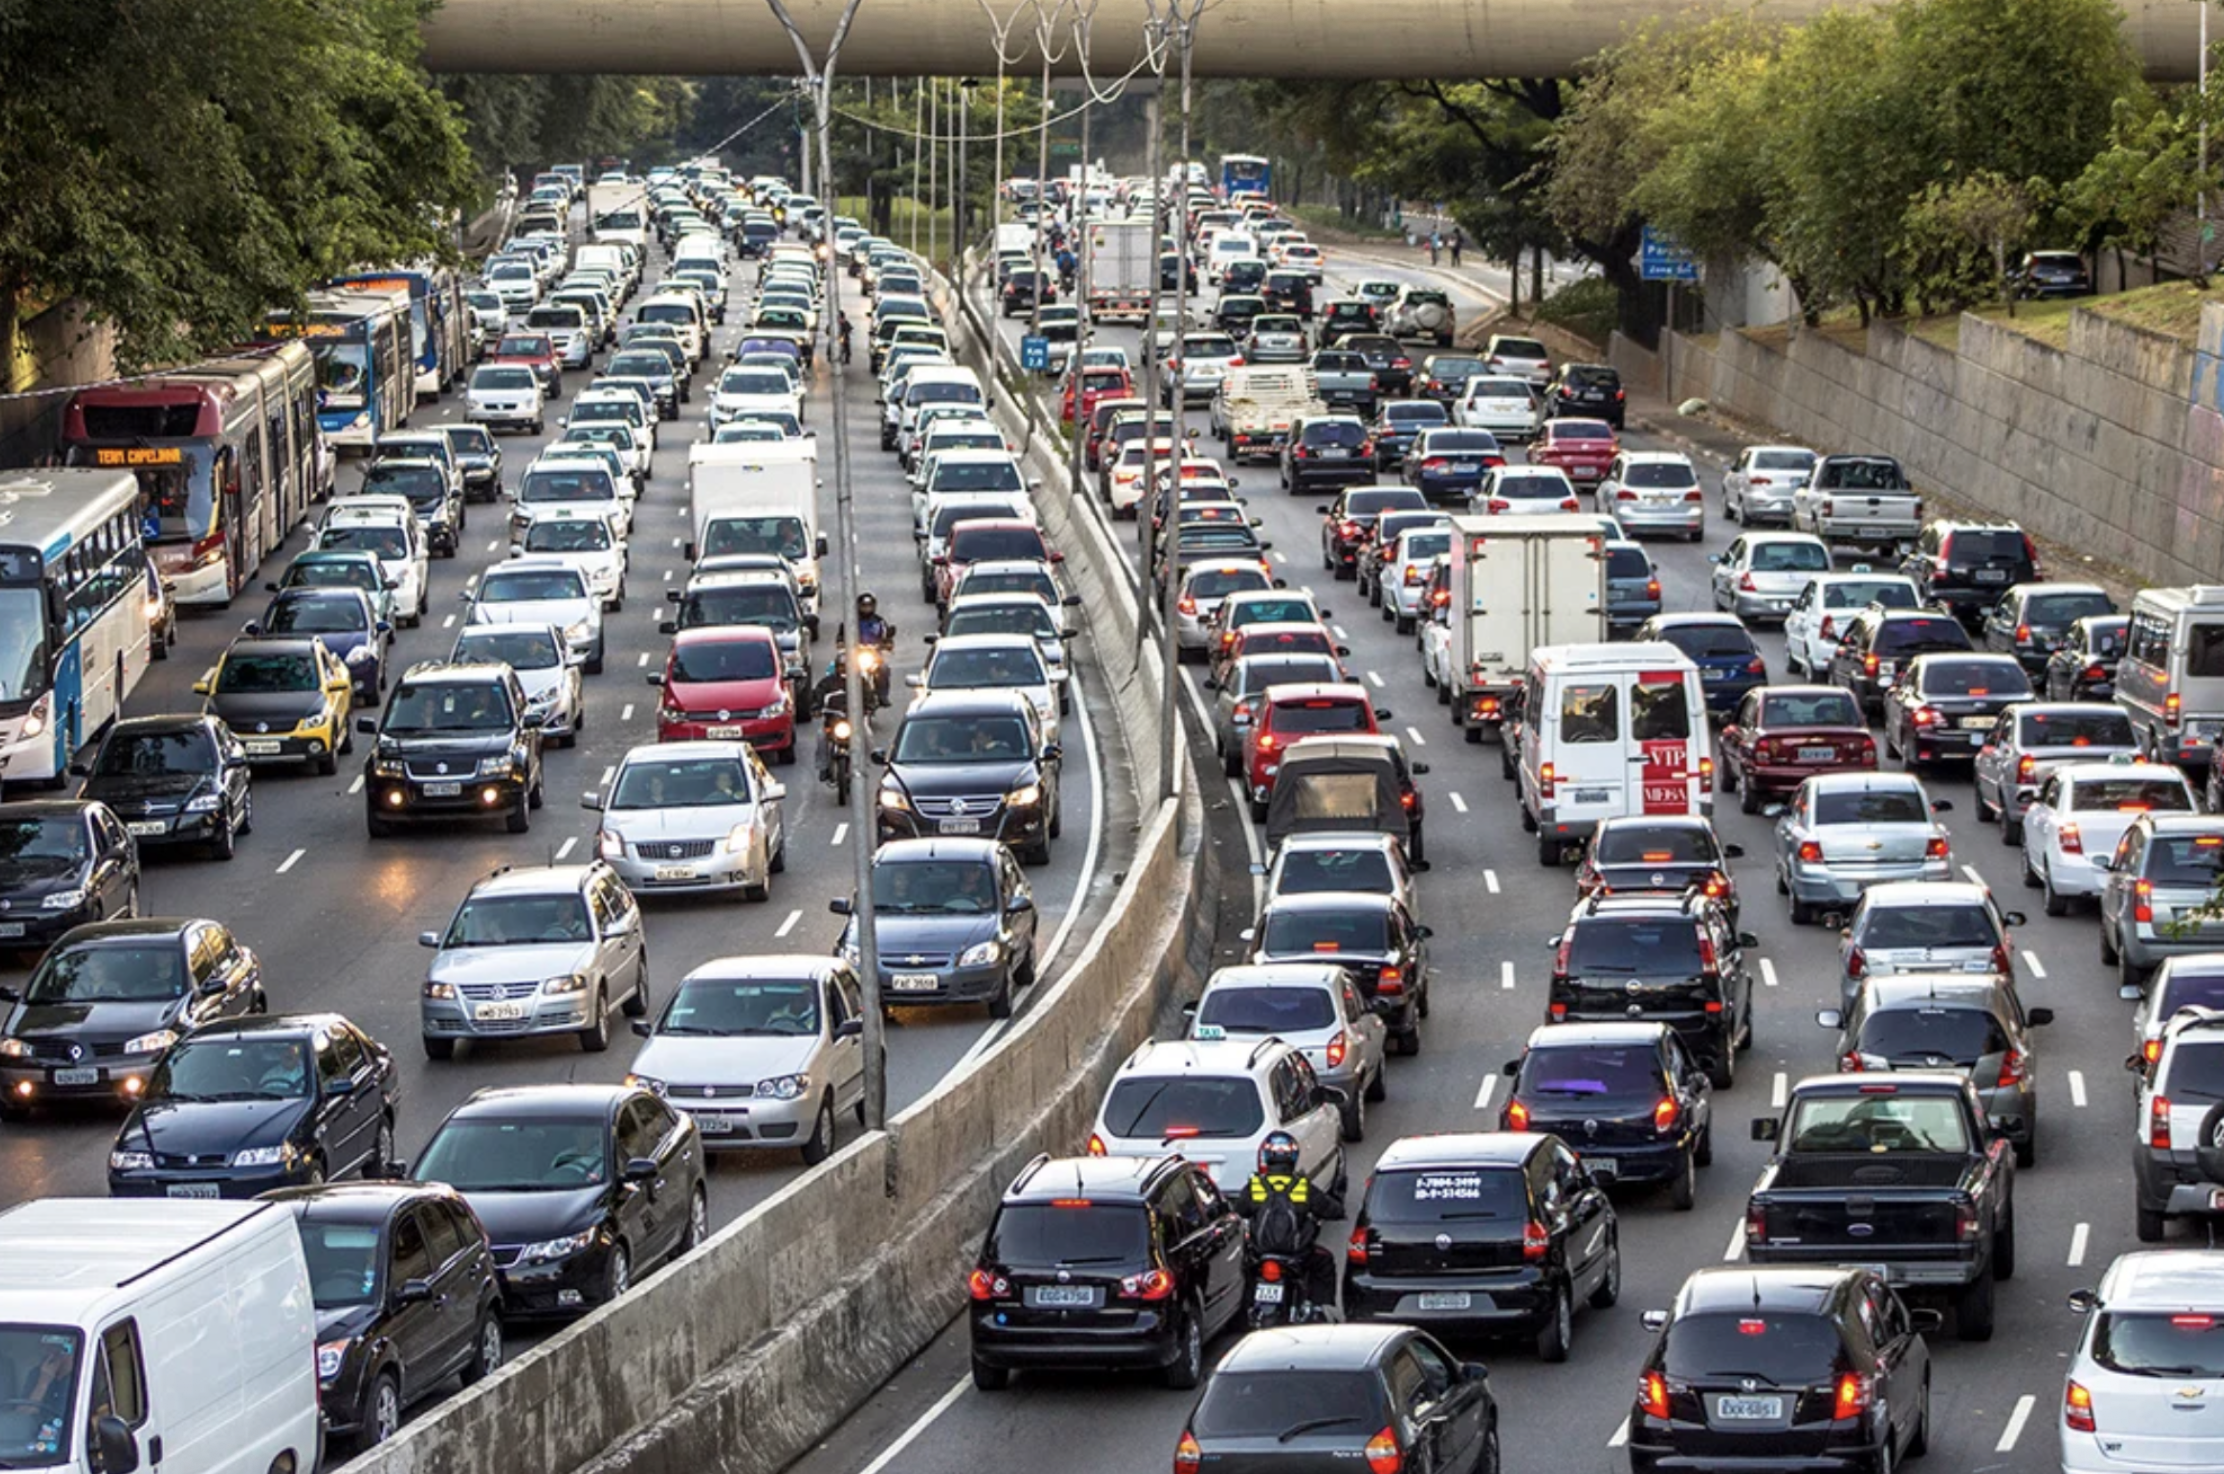
\includegraphics[width=0.6\textwidth]{assets/ch2/1.png}
    \caption{Camera Obscura principle.}
    \label{fig:camera_obscura}
\end{figure}

A simple setting for creating images on a white piece of paper is by projecting a shadow on it and, in the middle of the shadow, appears a picture of the scene in front of it. 

\begin{itemize}
    \item Leonardo da Vinci (1452-1519) was the first to describe the camera obscura in his notebooks.
    \item Johann Zahn (1685-1771) designed the first portable camera obscura in 1685.
    \item Joseph Nicephore Niepce (1765-1833) created the first permanent photograph in 1826 using a camera obscura.
\end{itemize}

\begin{minipage}{0.48\textwidth}
    From a geometrical point of view, the light rays of the object hit the film plane on different points, so we don't directly have the picture of the object. BUT, if we set a barrier in the middle, we have a one-to-one correspondence between the points of the object and the points of the film plane. That is why the pinhole camera works.
\end{minipage}
\hfill
\begin{minipage}{0.48\textwidth}
    \begin{figure}[H]
        \centering
        \includegraphics[width=0.8\textwidth]{assets/ch2/2.png}
        \caption{Pinhole camera principle.}
        \label{fig:pinhole_camera}
    \end{figure}
\end{minipage}

\begin{minipage}{0.48\textwidth}
    \begin{figure}[H]
        \centering
        \includegraphics[width=0.6\textwidth]{assets/ch2/3.png}
        \caption{Pinhole camera model.}
        \label{fig:pinhole_camera_model}
    \end{figure}
\end{minipage}
\hfill
\begin{minipage}{0.48\textwidth}
    \begin{itemize}
        \item The image is reversed upside-down and left-right;
        \item A \textit{virtual image} is formed in front of the camera.
    \end{itemize}
\end{minipage}

\paragraph{Perspective Projection} is composed by a \textit{principal plane}, parallel to the image plane and that contains the \textit{optical center ($C$)}. We then create the three axes, with the $Z$ one named \textit{principal axis}. 

\begin{figure}[H]
    \centering
    \includegraphics[width=\textwidth]{assets/ch2/4.png}
\end{figure}

Point $M$ is projected onto the image plane at point $M'$. By similarity of triangles, it follows that the 3D point $[X,Y,Z]^T$ is mapped to the point 
\[
[X',Y',Z']^T = \left[-\frac{f}{Z}X, -\frac{f}{Z}Y, -f\right]^T
\]
where $\frac{f}{Z}$ is the \textit{perspective scale factor}. Farther away objects (larger $Z$ appear smaller).

\paragraph{Weak Perspective} If the object is thin w.r.t. its distance from the camera, then the perspective scale factor is roughly constand:
\[
\frac{f}{Z_0 + \Delta Z} \approx \frac{f}{Z_0}
\]
Then, perspective projection can be approximated by a \textit{scaled orthographic projection}
\[
X' = -\frac{f}{Z_0}X, \quad Y' = -\frac{f}{Z_0}Y
\]
\begin{tipsblock}
    Rule of thumb due to Leonardo da Vinci: $\frac{\Delta Z}{Z_0} < \frac{1}{10}$
\end{tipsblock}

\begin{figure}[H]
    \centering
    \includegraphics[width=0.6\textwidth]{assets/ch2/5.png}
    \caption{Weak perspective projection.}
    \label{fig:weak_perspective}
\end{figure}

The \textbf{Aperture} is related to the amount of light that enters the camera. A larger aperture allows more light to enter, resulting in a brighter image. However, a larger aperture also reduces the depth of field, which is the range of distances within which objects appear sharp in the image.
\begin{itemize}
    \item \textbf{Pinhole too big} $\rightarrow$ many directions are averaged, blurring the image; bright but blurred image, because many directions are averaged;
    \item \textbf{Pinhole too small} $\rightarrow$ diffraction effects blur the image; sharp but dark image, because little light reaches the sensor.
\end{itemize}

\begin{figure}[H]
    \centering
    \includegraphics[width=0.8\textwidth]{assets/ch2/6.png}
    \caption{Aperture effects.}
    \label{fig:aperture_effects}
\end{figure}

Solution? \textbf{Lenses}!

\newpage
\subsection{Lenses}

A lens collects rays departing from the same points and focuses them onto the screen. There is a specific distance at which objects are in focus. Perspective projection is still valid within the thin lens assumption.

\begin{figure}[H]
    \centering
    \includegraphics[width=0.8\textwidth]{assets/ch2/7.png}
    \caption{Lens principle. The gray areas represent the set of rays originated from the object.}
    \label{fig:lens_principle}
\end{figure}

\begin{itemize}
    \item A \textit{thin lens} is composed of a single piece of glass with very low, equal curvature on both sides;
    \item Any ray that enters parallel to the axis on one side of the lens proceeds towards the \textbf{focal point $F$};
    \item Any ray that passes through the center of the lens $C$ does not change its direction;
    \item The distance $D$ from the center to the focal point is called \textbf{focal length $f$};
    \item The image $M'$ of $M$ can be found by intersecting two rays.
\end{itemize}

\begin{figure}[H]
    \centering
    \includegraphics[width=0.8\textwidth]{assets/ch2/8.png}
\end{figure}

Let's now try to use mathematical notation. Based on triangle similarity:
\[
\frac{Y'}{Y} = \frac{Z'}{Z}, \quad \frac{Y'}{Y} = \frac{Z' - D}{D}
\]
Thus, we get the \textbf{thin lens equation}, also known as the lensmaker's formula:
\[
\frac{1}{Z} + \frac{1}{Z'} = \frac{1}{D}
\]
which basically tells that points that are far away from the lens ($Z \to \infty$) are focused at the focal length ($Z' = D = f$).
Point $M$ is projected, when in focus, into the same position of a pinhole model having the optical center located in the lens center $C$.

\begin{minipage}{0.48\textwidth}
    \begin{itemize}
        \item Two points lying on opposite sides of the lens at distances that satisfy the thin lens equation are \textbf{conjugate points};
        \item In Figure \ref{fig:conjugate_points}, $A$ and $A'$ are conjugate;
        \item Parallel rays from infinity focus at distance $D$ from the lens;
        \item As a source of light rays moves closer to the lens, they focus further away on the other side;
        \item Rays originating from a point at a distance $D$ from the lens become parallel after passing throught the lens, i.e., they focus at infinity;
        \item To focus on objects at different distances, move sensor relative to the lens;
        \item at $Z = Z' = 2D$ we have $1 : 1$ imaging, since $\frac{1}{2D} + \frac{1}{2D} = \frac{1}{D}$;
        \item Can't focus on objects closer to the lens than its focal length $D$.
    \end{itemize}
\end{minipage}
\hfill
\begin{minipage}{0.48\textwidth}
    \begin{figure}[H]
        \centering
        \includegraphics[width=0.9\textwidth]{assets/ch2/9.png}
        \caption{Conjugate points.}
        \label{fig:conjugate_points}
    \end{figure}
\end{minipage}

\vspace{0.5cm}

The \textbf{field of view} of a camera is the portion of the scene space that actually projects onto the sensor. It depends on the focusing distance and on the sensor width $w$. Conventionally it is defined when focusing at infinity:
\[
f.o.v. = 2\phi = 2\arctan \frac{w}{2D}
\]

\begin{figure}[H]
    \centering
    \includegraphics[width=0.6\textwidth]{assets/ch2/10.png}
    \caption{Field of view.}
    \label{fig:field_of_view}
\end{figure}

\vspace{0.5cm}

The \textbf{blur circle} is the circle of confusion created when a point is not in focus. It is formed by rays and its size depends on $\Delta Z'$ and on the lens diameter $d$:
\[
\text{blur circle diameter} = d\frac{|\Delta Z'|}{Z'}
\]

The smaller the diameter, the smaller the blur circle, the sharper the image.

\begin{figure}
    \centering
    \includegraphics[width=\textwidth]{assets/ch2/11.png}
    \caption{Blur circle formation.}
    \label{fig:blur_circle}
\end{figure}

Once fixed the diameter of the blur circle, locate the farthest and the closest planes whose points are projected inside the blur circle: the distance between these planes is known as \textbf{depth of field}. Moreover, for a fixed diameter of the blur circle, the depth of field changes as the diameter of the lens (aperture) changes; in particular, the depth of field increases as the aperture decreases.

\begin{figure}[H]
    \centering
    \includegraphics[width=0.6\textwidth]{assets/ch2/12.png}
    \caption{Depth of field.}
    \label{fig:depth_of_field}
\end{figure}

\begin{observationblock}[Aperture size]
    The aperture size is usually expressed by the $f$-number, defined as
    \[
f\text{-number} = \frac{D}{d}
    \]
    where $D$ is the focal length and $d$ is the diameter of the aperture. Smaller $f$-numbers correspond to larger apertures, allowing more light to enter the camera, while larger $f$-numbers correspond to smaller apertures, reducing the amount of light.
\end{observationblock}

\newpage 

\begin{minipage}[t]{0.48\textwidth}
    \begin{figure}[H]
        \centering
        \includegraphics[width=0.9\textwidth]{assets/ch2/13.png}
        \caption{Lens aberrations.}
        \label{fig:lens_aberrations}
    \end{figure}
\end{minipage}
\hfill
\begin{minipage}[t]{0.48\textwidth}
    \vspace{0.5cm}
    Now, if we put a barrier with a hole in correspondence of the focus $F$, the light beams from $M$ are all blocked, except those parallel to the optical axis. The image of $M$ does not depend on $Z$ (depth), but only on $X$ and $Y$ and so the device performs an orthographic projection. This is a \textbf{Telecentric camera}.
\end{minipage}

Real (thick) lenses introduce several types of \textbf{aberrations} that cause deviations from the ideal pinhole camera model:
\begin{itemize}
    \item \textbf{Radial distortion} causes straight lines to appear curved in the image, especially towards the edges. It can be corrected using calibration techniques.
    \begin{itemize}
        \item \textbf{Barrel distortion} makes lines bulge outward from the center of the image.
        \item \textbf{Pincushion distortion} makes lines pinch inward towards the center of the image.
    \end{itemize}
    \item \textbf{Chromatic aberration} occurs because different wavelengths of light are focused at different points, leading to color fringing around high-contrast edges.
    \item \textbf{Spherical aberration} arises when light rays passing through the edges of a spherical lens focus at different points than those passing through the center, resulting in a blurred image.
\end{itemize}

\begin{figure}[H]
    \centering
    \includegraphics[width=0.8\textwidth]{assets/ch2/14.png}
    \caption{Examples of radial distortion}
    \label{fig:radial_distortion}
\end{figure}

\begin{figure}[H]
    \centering
    \includegraphics[width=0.8\textwidth]{assets/ch2/15.png}
    \caption{Example of chromatic aberration.}
    \label{fig:chromatic_aberration}
\end{figure}

\paragraph{Vignetting} is the darkening of image corners due to lens limitations or improper lens hoods. It can be corrected in post-processing. It is caused by \textit{compound lenses}, which may reduce aberrations but can introduce vignetting. In them, light beams emanating from object points located off-axis are partially blocked by individual lens components, resulting in a reduction of brightness toward the image periphery.
\begin{figure}[H]
    \centering
    \includegraphics[width=0.8\textwidth]{assets/ch2/16.png}
    \caption{Vignetting effect.}
    \label{fig:vignetting_effect}
\end{figure}

\paragraph{Sensing}, instead, is the process of converting the continuous image formed on the sensor into a discrete digital image. This involves sampling the continuous image at regular intervals (pixels) and quantizing the intensity values into discrete levels (bit depth). Since the sensor is a rectangular array of sensing elements (pixels), the image formed on the sensor is a rectangular portion of the image formed by the lens. The light charges a capacitor in each pixel, which is then read out and converted into a digital value. The longer the exposure time, the more light is collected, resulting in a brighter image. However, longer exposure times can also lead to motion blur if the camera or subject moves during the exposure. Finally, the capacitor is discharged periodically (the period is called \textit{shutter time}).

A simple sensor model is composed by:
\begin{itemize}
    \item an integrator that collects light over the exposure time $T$;
    \item a sampler that samples the integrated light at each pixel location;
    \item a quantizer that converts the sampled light intensity into discrete digital values.
\end{itemize}

Moreover, there are two approaches for sensing color:
\begin{itemize}
    \item the \textbf{3-sensor method}: a set of glass prisms uses a combination of internal reflection and refraction to split the incoming image into three, each reaching a different sensor;
    \item the \textbf{Bayer Mosaic}: half the pixels are sensitive to the green band of the light spectrum, while one quarter each to blue and red. This is consistent with the distribution of color-sensitive cones in the human retina. Color components that are not sensed (two per pixel), are inferred by interpolation from neighboring pixels.
\end{itemize}

\begin{figure}[H]
    \centering
    \includegraphics[width=0.6\textwidth]{assets/ch2/17.png}
    \caption{3-sensor beam splitter on the left, Bayer mosaic on the right.}
    \label{fig:color_sensing}
\end{figure}

\section{Camera Model}

The \textbf{simplified model} of a camera is based on the pinhole camera, where the image plane is placed in front of the pinhole to avoid the inversion of the image. 

\begin{minipage}{0.48\textwidth}
    \begin{figure}[H]
        \centering
        \includegraphics[width=0.6\textwidth]{assets/ch2/18.png}
        \caption{Simplified pinhole camera model.}
        \label{fig:simplified_pinhole_camera}
    \end{figure}
\end{minipage}
\hfill
\begin{minipage}{0.48\textwidth}
    \begin{itemize}
        \item $(X,Y,Z)$ is the world reference frame, centered in $\mathcal{C} \in \mathcal{F}$;
        \item The $Z$ axis corresponds to the optical axis;
        \item $(u,v)$ is the image frame, centered in the intersection between the optical axis and the image plane;
        \item $u$ and $v$ are oriented as $X$ and $Y$;
        \item The perspective projection is a map $\mathbb{R}^3 \to \mathbb{R}^2$ such that 
        \[
        (x,y,z) \rightarrow \left(-\frac{fx}{z}, -\frac{fy}{z}\right)
        \]
        \item The map is nonlinear (due to the division by $z$);
        \item A linear map can be recovered by using homogeneous coordinates.
    \end{itemize}
\end{minipage}

\textbf{Homogeneus coordinates} allow to add \textbf{improper points} (points ad infinite) to the usual Euclidean plane (or space). The basic idea is to represent a point $(x,y)$ of the plane as a triplet (u,v,w) of real numbers, in such a way that:
\[
x = \frac{u}{w} \quad \text{and} \quad y = \frac{v}{w}
\]
where $w \neq 0$. The triplet (u,v,w) is called the \textbf{homogeneous representation} of the point (x,y). The null triplet (0,0,0) does not represent any point. Moreover, any two triplets (u,v,w) and (ku,kv,kw), with $k \neq 0$, represent the same point (x,y).

\begin{definitionblock}[Projective plane]
    The \textbf{projective plane} $\mathbb{P}^2$ is the set of equivalence classes of non-zero triplets (u,v,w), where two triplets are equivalent if they differ by a non-zero scale factor $k$. 
    \[
    (u,v,w) \sim \lambda(u,v,w) \quad \forall \lambda \neq 0
    \]
    The projective plane includes all points in the Euclidean plane (where $w \neq 0$) as well as points at infinity (where $w = 0$).
\end{definitionblock}

A similar definition holds for the \textbf{projective space} $\mathbb{P}^3$, where points are represented by quadruplets (X,Y,Z,W) and two quadruplets are equivalent if they differ by a non-zero scale factor $k$.

\begin{exampleblock}
    Consider the vector $(x',y',0)$. We have points that specify a direction but are at an infinite distance from focal point. So,
    \[
    \begin{pmatrix}
    x' \\
    y' \\
    0
    \end{pmatrix} \to \begin{pmatrix}
    \frac{x'}{0} \\ 
    \frac{y'}{0} \\
    \end{pmatrix} \to \begin{pmatrix}
    \infty \\
    \infty
    \end{pmatrix}
    \]
    Points whose last coordinate is zero are said to be \textbf{improper}.
\end{exampleblock}

Improper points represent a point at infinite along a direction specified by the non-zero coordinates. Points whose last coordinate is not zero, are said to be \textbf{proper}. To represent them, we can simply "add" a coordinate. With no loss of generality it may be taken as equal to 1, obtaining the so called \textbf{augmented vector}.
\[
(x,y) \to \begin{bmatrix}
x \\
y \\
1
\end{bmatrix}
\quad 
(x,y,z) \to \begin{bmatrix}
x \\
y \\
z \\
1
\end{bmatrix}
\] 

Converting from homogeneus coordinates to Cartesian coordinates is called \textbf{dehomogenization} and amounts to dividing by the last coordinate:
\[
\begin{bmatrix}
u \\
v \\
w
\end{bmatrix} \to \begin{bmatrix}
\frac{u}{w} \\
\frac{v}{w}
\end{bmatrix}
\to
\begin{bmatrix} 
\frac{u}{w} \\
\frac{v}{w} \\
1
\end{bmatrix}
\]

\subsection{Transformations} 
Let the augmented vector corresponding to $x$ be denoted by $\bar{x}$. 
\begin{itemize}
    \item \textbf{Translation}: a translation of $t$ may be written as 
    \[
    x' = x + t 
    \]
    or 
    \[
    x' = \left[I | t\right]\bar{x}
    \] 
    or 
    \[
    \bar{x}' = \begin{bmatrix}
    I & t \\
    0^T & 1
\end{bmatrix} \bar{x}
    \]   
    \item \textbf{Rotation and translation} (rigid body motion):
    \[
    x' = Rx + t 
    \]
    or 
    \[
    x' = \left[R | t\right]\bar{x}
    \]
    or
    \[
    \bar{x}' = \begin{bmatrix}
    R & t \\
    0^T & 1
\end{bmatrix} \bar{x}
    \]
    where $R$ is an orthonormal matrix, thus $RR^T = R^TR = I$ and $\det(R) = 1$. 
    \begin{observationblock}
        There is also $\det(R) = -1$, which encodes a \textbf{mirroring} effect, not allowed in rigid transformations.
    \end{observationblock}
    In the 2D case, given the angle $\theta$ of rotation, $R$ takes the form 
    \[R = \begin{bmatrix}
    \cos \theta & -\sin \theta \\
    \sin \theta & \cos \theta
    \end{bmatrix}\]
    where $R$ is a rotation matrix.
    \item \textbf{Similarity transformation} (where $s$ is the scale factor):
    \[
    x' = sRx + t 
    \]
    or 
    \[
    x' = \left[sR | t\right]\bar{x}
    \]
    or
    \[
    \bar{x}' = \begin{bmatrix}
    sR & t \\
    0^T & 1
\end{bmatrix} \bar{x}
    \]
\end{itemize}

\begin{figure}[H]
    \centering
    \includegraphics[width=0.9\textwidth]{assets/ch2/19.png}
    \caption{2D Transformations}
    \label{fig:transformations}
\end{figure}

Let $m$ and $m'$ be the vectors of homogeneous coordinates of $M$ (w.r.t. the camera frame) and $M'$ (w.r.t. the image frame):
\[
m = \begin{bmatrix}
x \\
y \\
z \\
1
\end{bmatrix}, \quad
m' = \begin{bmatrix}
u \\
v \\
1
\end{bmatrix}
\]
Then 
\[
z \begin{bmatrix}
u \\
v \\    
1
\end{bmatrix} = z \begin{bmatrix}
    -\frac{fx}{z} \\ 
    -\frac{fy}{z} \\
    1
\end{bmatrix} = \begin{bmatrix}
    -fx \\ 
    -fy \\
    z
\end{bmatrix} = \underbrace{\begin{bmatrix}
    -f & 0 & 0 & 0 \\
    0 & -f & 0 & 0 \\
    0 & 0 & 1 & 0 \\
\end{bmatrix}}_{\text{Projection Matrix}} \begin{bmatrix}
x \\
y \\
z \\
1
\end{bmatrix}
\]

Thus, in matrix notation 
\[
m' = \frac{1}{z} Pm 
\]

or equivalently 
\[
m' \sim Pm
\]
where $\sim$ means equality up to a scale factor.

\subsection{General Model}
\begin{minipage}{0.48\textwidth}
    For a more general camera model we need to consider:
    \begin{itemize}
        \item the rigid transformation from the world reference frame to the camera frame;
        \item the \textbf{pixelization} (from meters to pixel, in the image reference frame);
        \item The pixelization amounts to a \textbf{rescaling} followed by a translation:
        \[
        V = \begin{bmatrix}
            -k_u & 0 & u_0 \\ 
            0 & -k_v & v_0 \\
            0 & 0 & 1 \\
        \end{bmatrix}
        \]
        where $(u_0, v_0)$ are the coordinates (in pixels) of $\mathcal{C'}$;
        \item $k_u$ and $k_v$ the reciprocal of the pixel size along $u$ and $v$:
        \[
        k_u = \frac{1}{s_u} \quad k_v = \frac{1}{s_v} \quad \left[\text{pixel}\times m^{-1}\right]
        \]
    \end{itemize}
\end{minipage}
\hfill
\begin{minipage}{0.48\textwidth}
    \begin{figure}[H]
        \centering
        \includegraphics[width=0.9\textwidth]{assets/ch2/20.png}
        \caption{General camera model.}
        \label{fig:general_camera_model}
    \end{figure}
\end{minipage}

\vspace{0.5cm}

Thus the new $P$ taking into account the sensor is:
\[
P = \begin{bmatrix}
    -k_u & 0 & u_0 \\
    0 & -k_v & v_0 \\
    0 & 0 & 1 \\
\end{bmatrix} \begin{bmatrix}
    -f & 0 & 0 & 0 \\
    0 & -f & 0 & 0 \\
    0 & 0 & 1 & 0 \\
\end{bmatrix} = \begin{bmatrix}
    f k_u & 0 & -u_0 & 0 \\
    0 & f k_v & -v_0 & 0 \\
    0 & 0 & 1 & 0 \\
\end{bmatrix} = K\left[I | 0\right]
\]
where, by posing $fk_u = \alpha_u$ and $fk_v = \alpha_v$, we have 
\[
K = \begin{bmatrix}
    \alpha_u & 0 & u_0 \\
    0 & \alpha_v & v_0 \\
    0 & 0 & 1 \\
\end{bmatrix} \quad \text{and} \quad \left[I | 0\right] = \begin{bmatrix}
    1 & 0 & 0 & 0 \\
    0 & 1 & 0 & 0 \\
    0 & 0 & 1 & 0 \\
\end{bmatrix}
\]

\begin{itemize}
    \item $K$ is the \textbf{calibration matrix};
    \item $K$ describes the camera intrinsics (those parameters that depend on the camera itself, as opposite to the camera's pose in space, which are called extrinsics);
    \item Notice that $K$ is upper triangular.
\end{itemize}

Let's now take into account the rigid transformation from the world reference frame to the camera frame and the pixelization. Let $m_c$ be the vector of homogeneous coordinates of $M$ with respect to the camera reference frame and let 
\[
G = \begin{bmatrix}
    R & t \\
    0^T & 1 \\
\end{bmatrix}
\]
be the rigid body motion from the world frame to the camera frame (a rotation $R$ followed by a translation $t$). It follows that 
\[
m_c = G m
\]
The matrix $G$ represents the camera extrinsics. The perspective projection is thus:
\[
m' \sim K\left[I | 0\right] Gm 
\]
The perspective projection matrix in the general case is 
\[
P = K\left[I | 0\right] G = K\left[R | t\right]
\]
By partitioning $R$ and $t$ row-wise:
\[
R = \begin{bmatrix}
r_1^T \\
r_2^T \\
r_3^T \\
\end{bmatrix}, \quad t = \begin{bmatrix}
t_1 \\
t_2 \\
t_3 \\
\end{bmatrix}
\]
we obtain 
\[
P = \begin{bmatrix}
    \alpha_u r_1^T + u_0 r_3^T & \alpha_u t_1 + u_0 t_3 \\
    \alpha_v r_2^T + v_0 r_3^T & \alpha_v t_2 + v_0 t_3 \\
    r_3^T & t_3 \\
\end{bmatrix}
\]

\begin{observationblock}
    \begin{enumerate}
        \item A more general form of $K$ takes into account a further intrinsic parameter (the skew angle between the $u$ and $v$ axes, usually very close to $\frac{\pi}{2}$), thus 
        \[
K = \begin{bmatrix}
    \alpha_u & \alpha_u \cot \theta & u_0 \\
    0 & \frac{\alpha_v}{\sin \theta} & v_0 \\
    0 & 0 & 1 \\
\end{bmatrix}
        \]
        \item $P$ is defined up to a scale factor (for $\lambda \neq 0$, $\lambda P$ results in the same projection as $P$). A prospective projection matrix is said to be \textit{normalized} if has the form 
        \[
        \begin{bmatrix}
            * & * & * & \vline & * \\
            * & * & * & \vline & * \\
            \hline
            & a^T & & \vline & * \\
        \end{bmatrix}
        \]
        \item $P$ has 12 entries, but (due to the scale factor) 11 degrees of freedom. Indeed, it depends on $6+5=11$ independent parameters (6 extrinsic and 5 intrinsic).
        \item Partitioning $P$ row-wise
        \[
        P = \begin{bmatrix}
            p_1^T \\
            p_2^T \\
            p_3^T \\
        \end{bmatrix}
        \]
        we get 
        \[
        m' = Pm = \begin{bmatrix}
            p_1^T m \\
            p_2^T m \\
            p_3^T m \\
        \end{bmatrix} \rightarrow^{\text{back to inhomogeneous}} \begin{cases}
            u = \frac{p_1^T m}{p_3^T m} \\
            v = \frac{p_2^T m}{p_3^T m} \\
        \end{cases}
        \]
        where $u$ and $v$ are the Cartesian coordinates of point $M'$ in the image plane. Thus the last pair or equations is the generalization of the basic perspective projection equations.
    \end{enumerate}
\end{observationblock}

\newtheorem{theorem}{Theorem}
\begin{theorem}
    Let $P = \left[Q | q\right]$ be $3\times 4$ matrix and let $q_i^t, i=1,2,3$ denote the rows of $Q$.
    \begin{itemize}
        \item A necessary and sufficient condition for $P$ to be a perspective projection matrix is that 
        \[
        \det(Q) \neq 0
        \]
        \item A necessary and sufficient condition for $P$ to be a zero-skew perspective projection matrix is that 
        \[
        \det(Q) \neq 0 \quad \text{and} \quad (q_1 \times q_3)^T(q_2 \times q_3) = 0
        \]
    \end{itemize}
\end{theorem}

\subsection*{Center of Projection}

\begin{minipage}{0.48\textwidth}
    The focal plane $\mathcal{F}$ contains the points that are projected to the infinite (because the straight line through $C$ does not intersect the image plane). Thus its equation is
    \[
    p_3^T x = 0
    \]
    This is the equation of the focal plane and all points that satisfy it are in the focal plane, meaning that their projection goes to infinity. The planes $p_1^T x = 0$ and $p_2^T x = 0$ project to the axes $u = 0$ and $v = 0$, respectively. 

    The center of projection $C$ belongs to all the three planes, thus it is defined by 
\end{minipage}
\hfill
\begin{minipage}{0.48\textwidth}
    \begin{figure}[H]
        \centering
        \includegraphics[width=0.7\textwidth]{assets/ch2/21.png}
        \caption{Center of projection.}
        \label{fig:center_of_projection}    
    \end{figure}
\end{minipage}

\[
\begin{cases}
p_1^T x = 0 \\
p_2^T x = 0 \\
p_3^T x = 0 \\
\end{cases}
\]
In other words, $C$ is represented (in homogeneous coordinates) by the kernel of $P$. 

$P$ has rank 3 by construction (both $K$ and $R$ are invertible) hence, by the Rank-Nullity Theorem 
\[
\text{dim}(\text{Ker}(P)) = 4 - \text{rank}(P) = 4 - 3 = 1
\]
Let
\[
\tilde{c} = \left[x_C y_C z_C\right]^t
\]
be the vector of the Cartesian coordiantes of $C$ w.r.t. the world frame. We can write 
\[
P_c = \left[Q | q\right] \begin{bmatrix}
\tilde{c} \\
1
\end{bmatrix} = 0
\]
then, solving for $\tilde{c}$ we get
\[
\tilde{c} = -Q^{-1} q
\]

\subsection*{Optical Ray}
\begin{minipage}{0.48\textwidth}
    The optical ray of an image point $M'$ is the locus of points in space that project onto $M'$. May be expressed as the line through $C$ and a point $\alpha$ located at infinity that projects onto $M'$ 
    \[
\alpha = \begin{bmatrix}
    Q^{-1} m' \\
    0
    \end{bmatrix}
    \]
    thus a parametrics representation (in homogeneous coordinates) of the optical ray is 
    \[
    m = c + \lambda\begin{bmatrix}
    Q^{-1} m' \\
    0
    \end{bmatrix}, \quad \lambda \in \mathbb{R}
    \]
\end{minipage}
\hfill
\begin{minipage}{0.48\textwidth}
    \begin{figure}[H]
        \centering
        \includegraphics[width=0.7\textwidth]{assets/ch2/22.png}
        \caption{Optical ray.}
        \label{fig:optical_ray}
    \end{figure}
\end{minipage}

\begin{advancedblock}[Depth of a point]
    Consider a point $M$ whose Cartesian coordinates w.r.t. the world reference frame are $\tilde{m} = \left[x_M y_M z_M\right]^T$. The projection equation with explicit scale factor $\zeta$ is 
    \[
    \zeta m' = Pm 
    \]
    Representing $M$ in homogeneous coordinates as $m = \left[\tilde{m}^T 1\right]^T$ we get 
    \[
    \begin{bmatrix}
    \zeta u \\
    \zeta v \\
    \zeta z \\
    \end{bmatrix} = P \begin{bmatrix}
        \tilde{m} \\    
        1 \\
    \end{bmatrix} 
    \]
    If $P$ is normalized, we obtain, from the third scalar equation, that
    \[
    \zeta = r_3^T \tilde{m} + t_3
    \]
    Recalling that $m_c = Gm$, it follows that $\zeta$ is the third coordinate of $M$ w.r.t. the camera frame or the distance from $M$ to the focal plane (depth of the point $M$). In other words, if
    \begin{enumerate}
        \item the last homogeneous coordinate is chosen as 1;
        \item $P$ is normalized;
    \end{enumerate}
    then the last homogeneous projected coordinate $\zeta$ is the depth of the point. 
\end{advancedblock}

\section{Camera Calibration}

\begin{figure}[H]
    \centering
    \includegraphics[width=0.8\textwidth]{assets/ch2/23.png}
    \caption{Camera calibration.}
    \label{fig:camera_calibration}
\end{figure}

Camera calibration is the process of estimating the intrinsic and extrinsic parameters of a camera. This is typically done by capturing images of a known calibration pattern (e.g., a checkerboard) from different viewpoints and using these images to solve for the camera parameters.
\begin{itemize}
    \item \textbf{Camera calibration problem}: estimate intrinsic and extrinsic camera parameters, based on some measurements;
    \item \textbf{Calibration pattern}: a 3D object of known geometry and generating image features which can be located accurately;
    \item Parameters may be estimated based on a set of known 3D-2D correspondences;
    \item \textbf{Direct methods}: formulate a problem in which the camera parameters are the unknowns;
    \item \textbf{Indirect methods}: first estimate the projection matrix $P$ and then decompose it to get intrinsic and extrinsic parameters.
\end{itemize}

\newpage 
\subsection{Direct Linear Transform}

This is an indirect method. Suppose having $n$ correspondences 
\[
m_{(i)} = \begin{bmatrix}
x_{(i)} \\
y_{(i)} \\
z_{(i)} \\
1
\end{bmatrix} \quad \text{and} \quad m'_{(i)} = \begin{bmatrix}
u_{(i)} \\
v_{(i)} \\
1
\end{bmatrix} \quad i = 1, \ldots, n
\]

For each correspondence, two scalar equations hold 
\[
\begin{cases}
u_{(i)} = \frac{p_1^T m_{(i)}}{p_3^T m_{(i)}} \\
v_{(i)} = \frac{p_2^T m_{(i)}}{p_3^T m_{(i)}} \\
\end{cases} \quad \to \quad \begin{cases}
m_{(i)}^T \overbrace{p_1}^{\text{transpose of 1st row}} - u_{(i)}m_{(i)}^T p_3 = 0 \\
m_{(i)}^T \overbrace{p_2}^{\text{transpose of 2nd row}} - v_{(i)}m_{(i)}^T p_3 = 0 \\
\end{cases}
\]

\begin{tipsblock}
Remember that when applying a transposition or an inversion, the following properties hold:
\begin{itemize}
    \item $(AB)^T = B^T A^T$;
    \item $(A^T)^{-1} = (A^{-1})^T$.
\end{itemize}
\end{tipsblock}

Thus, in a more compact form:
\[
\underbrace{\begin{bmatrix}
m_{(i)}^T & 0^T & -u_{(i)} m_{(i)}^T \\
0^T & m_{(i)}^T & -v_{(i)} m_{(i)}^T \\
\end{bmatrix}}_{\text{A (knowns)}} \underbrace{\begin{bmatrix}
p_1 \\
p_2 \\
p_3 \\
\end{bmatrix}}_{\text{P (unknowns)}} = 0
\]

By stacking the $n$ pairs of equations we get an \textbf{homogeneous linear system} of $2n$ equations in 12 unkowns (entries of $P$). 
We then have a $2n \times 12$ coefficient matrix $A$ where at least $n=6$ points are needed to compute $P$. In general, and in absense of measuring errors, $A$ has rank 11, and the solution is the null-space of $A$. 
In practice, $A$ will be full-rank and $b$ can be estimated by solving the following optimization problem:
\[
\argmin{||p||=1} ||Ap||^2
\]
where the constraint forces to discard the trivial solution $p=0$ (which is not acceptable since $P \neq 0$). Notice that since $P$ is defined up to a scale factor, any constraint of the form $||p||=\lambda \neq 0$ will result in the same actual estimated projection. 

The solution of the minimization problem is the right singular vector of $A$ corresponding to the smallest singular value. If 
\[
A = U\Sigma V^T 
\]
then $p = v_{12}$, i.e. the rightmost column of $V$.

\begin{observationblock}
    We expect $rank(A) \leq 11$, but in practice (due to the noise) we usually get 12. There is thus no exact solution except for 0, but it is not acceptable by default.
\end{observationblock}

The \textbf{cross product} $a\times b$ is a vector defined as 
\[
a \times b = \begin{bmatrix}
\det\begin{bmatrix}a_2 & a_3 \\
b_2 & b_3\end{bmatrix} \\
-\det\begin{bmatrix}a_1 & a_3 \\
b_1 & b_3\end{bmatrix} \\
\det\begin{bmatrix}a_1 & a_2 \\
b_1 & b_2\end{bmatrix}
\end{bmatrix}
\]
It is null if and only if $b = \lambda a$ for any scalar $\lambda$. It may be obtained as a matrix multiplication with a skew-symmetric matrix. Let 
\[
[a]_{\times} = \begin{bmatrix}
0 & -a_3 & a_2 \\
a_3 & 0 & -a_1 \\
-a_2 & a_1 & 0 \\
\end{bmatrix}
\]
then $[a]_{\times} b = 0$ if and only if $b = \lambda a$.

\begin{figure}[H]
    \centering
    \includegraphics[width=0.4\textwidth]{assets/ch2/24.png}
    \caption{Cross product geometric interpretation.}
    \label{fig:cross_product}
\end{figure}

\begin{definitionblock}[Kronecker product]
    Given the matrices $A^{m\times n}$ and $B^{p\times q}$, their \textbf{Kronecker product} $A \otimes B$ is the matrix of size $(mp) \times (nq)$ defined as
    \[
    A \otimes B = \begin{bmatrix}
    a_{11}B & a_{12}B & \ldots & a_{1n}B \\
    a_{21}B & a_{22}B & \ldots & a_{2n}B \\
    \vdots & \vdots & \ddots & \vdots \\
    a_{m1}B & a_{m2}B & \ldots & a_{mn}B \\
    \end{bmatrix}
    \]
\end{definitionblock}

This product is defined for any pair of matrices, is non commutative and enjoys the following properties:
\begin{itemize}
    \item $(A\otimes B)\otimes C = A\otimes (B\otimes C)$;
    \item $(A\otimes B)^T = A^T \otimes B^T$;
    \item $(A\otimes B)^{-1} = A^{-1} \otimes B^{-1}$;
    \item For square $A$ and $B$: if $\lambda_A$ is an eigenvalue of $A$ and $\lambda_B$ is an eigenvalue of $B$, then $\lambda_A \lambda_B$ is an eigenvalue of $A\otimes B$;
    \item $rank(A\otimes B) = rank(A) \times rank(B)$.
\end{itemize}

\begin{definitionblock}[Vector Operator]
    Given a matrix $X = \left[x_1 x_2 \dots x_n\right]$, the \textbf{vector operator} $vec$ is the operator that stacks the columns one underneath the other to a single vector:
    \[
    vec(X) = \begin{bmatrix}
    x_1 \\
    x_2 \\
    \vdots \\
    x_n \\
    \end{bmatrix}
    \]
\end{definitionblock}

The following identity holds:
\[
vec(AXB) = (B^T \otimes A) vec(X)
\]

and is used to "pull out" the unknown $X$ from a matrix equation.

For square matrices, the $vech$ (vector half) operator turns out to be useful:
\begin{definitionblock}[Vector Half Operator]
    Given a square matrix $X = \left[x_1 x_2 \dots x_n\right]$, the \textbf{vector half operator} (vech) is the operator that stacks in a single column the elements of $X$, which are on or below the diagonal, taken in column-wise order. Thus, $vech(X)$ has $n(n+1)/2$ elements. 
\end{definitionblock}

The projection equation states that:
\[
m_{(i)}' \sim P m_{(i)}
\]
and taking the product of both sides by the vector $Pm_{(i)}$ we get:
\[
m_{(i)}' \times (P m_{(i)}) = 0
\]
Thus we can get rid of the arbitrary scale factor and write:
\[
m_{(i)}' \times Pm_{(i)} = 0
\]
that is equivalent to 
\[
\left[m_{(i)}'\right]_{\times} P m_{(i)} = 0
\]
and by transposing, to
\[
m_{(i)}^T P^T \left[m_{(i)}'\right]_{\times}^T = 0^T
\]
Then, by applying the vector operator to both sides, and recalling that 
\[
vec(AXB) = \left(B^T\otimes A\right)vec(X)
\]
we obtain a triplet of linear equations in the unknown $vec(P^T)$:
\[
\left(\left[m_{(i)}'\right]_{\times}\otimes m_{(i)}^T\right)vec(P^T) = 0
\]
or, by expanding the coefficients:
\[
\begin{bmatrix}
0^T & -m_{(i)}^T & v_{(i)}m_{(i)}^T \\
m_{(i)}^T & 0^T & -u_{(i)}m_{(i)}^T \\
-v_{(i)}m_{(i)}^T & u_{(i)}m_{(i)}^T & 0^T \\
\end{bmatrix} vec(P^T) = 0
\]
Notice that only two equations are independent since the Kronecker product ($\left[m_{(i)}'\right]_{\times}\otimes m_{(i)}^T$) is rank two. 

For random configurations of $n\geq 6$ points, $A$ will have rank 11 or 12. In either case, a unique solution can be found (up to a scale factor). The \textbf{degenerate configurations} are those for which $P$ cannote be uniquely determined. 
\[
dim(ker(A))\geq 2 \quad \to \quad rank(A) \leq 10
\]

meaning that the space of solutions has dimension greater than one. The most important degenerate configurations are:
\begin{itemize}
    \item the points all lie on the union of a plane and a single straight line containing the camera center;
    \item the camera and the points all lie on a twisted cubic passing through the origin.
\end{itemize}

\begin{tipsblock}
    In practice, don't take more than six non-coplanar points. 
\end{tipsblock}

So, DLT minimizes the algebraic residual $||Ap||^2$, which has no geometrical meaning and is not invariant with respect to changes of the reference frame. Instead, the \textbf{geometric residual}:
\[
\epsilon(P) = \sum_{i=1}^n\left(\frac{p_1^T m_{(i)}}{p_3^T m_{(i)}} - u_{(i)}\right)^2 + \left(\frac{p_2^T m_{(i)}}{p_3^T m_{(i)}} - v_{(i)}\right)^2
\]
best expresses the actual need, that is to minimize the reprojection error (the distance between the estimated and the measured projections).
The resulting non-linear optimization problem can be solved iteratively, starting from an initial guess obtained via the DLT.

Given the estimated perspective projection matrix $P$, the intrinsic and extrinsic camera parameters can be computed as follows. 
The matrix $P$ is given in the form 
\[
P = \left[Q|q\right]
\]
where $Q$ is \textbf{invertible}. We want to express $P$ as 
\[
P = K\left[R | t\right] = \left[KR | Kt\right] 
\] 
where $K$ is upper triangular and $R$ is orthogonal. Thus, 
\[
Q = KR \quad \text{and} \quad q = Kt
\]

Recalling that any real square matrix can be written as the product of an orthogonal matrix and an upper triangular matrix, and letting $Q^{-1} = US$ be the QR factorization of $Q^{-1}$, we can write:
\[
Q = S^{-1}U^{-1}
\]
where $S^{-1}$ is upper triangular being the inverse of an upper triangular matrix, and $U^{-1}$ is orthogonal as $U$ is orthogonal. Hence a solution is:
\[
R = U^{-1},\quad K = S^{-1}, \quad t = K^{-1} q
\]
\begin{observationblock}
    Note that $P$ may contain an arbitrary scale factor that will affect $K$. The proper scale for $K$ is obtained by imposing $K_{33} = 1$.
\end{observationblock}

A further observation is that it is not possible to recover the "true" focal length $f$ from the 3D-2D correspondences only (without knowing the actual sensor size or the pixel size). Indeed, recalling that the calibration matrix $K$ takes the form 
\[
K = \begin{bmatrix}
    \alpha_u & \alpha_u \cot \theta & u_0 \\
    0 & \frac{\alpha_v}{\sin \theta} & v_0 \\
    0 & 0 & 1 \\
\end{bmatrix} = \begin{bmatrix}
    fk_u & fk_u \cot \theta & u_0 \\
    0 & \frac{fk_v}{\sin \theta} & v_0 \\
    0 & 0 & 1 \\
\end{bmatrix}
\]
where $k_u$ and $K_v$ are the reciprocal of the pixel sizes, along $u$ and $v$ respectively, it is clear that $f$ is "entangled" with $k_u$ and $k_v$. Thus, without knowing the pixel sizes, it is not possible to separate $f$ from them. If we, for instance, double the focal length as well as the pixel sizes we get the same calibration matrix. Thus, we can only recover $\alpha_u$ and $\alpha_v$.

\begin{advancedblock}[Dealing with radial distortion]

\end{advancedblock}

\subsection{Zhang's method}

Since DLT calibration requires an image of many ($\geq 6$) non co-planar points, and so building an accurate 3D calibration object may be difficult, we can use an easier method that requires $\geq 3$ images of a plane and is based on \textit{homography}: the \textbf{Zang's calibration method}.

\begin{definitionblock}[Homography]
    A \textbf{homography} is an isomorphism of $P^n$, i.e., a map 
    \[
    x\to Hx, \quad H^{(n+1)\times(n+1)}, \text{ non-singular}
    \]
    where $H$ and $\lambda H, \lambda \neq 0$ represent the same homography. 
\end{definitionblock}

\begin{figure}[H]
    \centering
    \includegraphics[width=0.5\textwidth]{assets/ch2/25.png}
    \caption{Homography mapping between two planes.}
    \label{fig:homography}
\end{figure}

The map from a 3D plane $\pi$ to its perspective image is easily seen to be a homography. Assume for simplicity that the plane has equation $z=0$. Then 
\[
w\begin{bmatrix}
    u \\
    v \\
    1
\end{bmatrix} = P \begin{bmatrix}
    x \\
    y \\
    0 \\
    1
\end{bmatrix} = \begin{bmatrix}
    p_1 & p_2 & p_3 & p_4 \\
\end{bmatrix} \begin{bmatrix}
    x \\
    y \\
    0 \\
    1
\end{bmatrix} = \underbrace{\begin{bmatrix}
    p_1 & p_2 & p_4 \\
\end{bmatrix}}_{=H} \begin{bmatrix}
    x \\
    y \\
    1
\end{bmatrix}
\] 
where the matrix $H$ is non-singular unless for degenerate cases. Given at least 4 pairs of original and projected points, a matrix $H$ corresponding to a homography can be computed via DLT. 

Suppose a homography $H$ of a 3D plane $\pi$ to the image plane is known (e.g. estimated from measurements):
\[
H = \lambda\begin{bmatrix}
    p_1 & p_2 & p_4 \\
\end{bmatrix}
\]
Since $P = K\left[R|t\right] = K\begin{bmatrix} r_1 & r_2 & r_3 & t\end{bmatrix}$, we get $p_1 = K r_1$, $p_2 = K r_2$ and $p_4 = Kt$. Then, by substitution:
\[
H = \lambda K \begin{bmatrix}
    r_1 & r_2 & t 
\end{bmatrix}
\]

Thus:
\[
\begin{cases}
    h_1 = \lambda K r_1 \\
    h_2 = \lambda K r_2 \\
\end{cases} \to \begin{cases}
    r_1 = \frac{1}{\lambda} K^{-1} h_1 \\
    r_2 = \frac{1}{\lambda} K^{-1} h_2 \\
\end{cases}
\]
Now, being $R$ a rotation matrix, we have 
\[
\begin{cases}
    r_1^T r_2 = 0 \\
    r_1^T r_1 = r_2^T r_2 = 1 \\
\end{cases} \to \begin{cases}
    h_1^T(KK^T)^{-1}h_2 = 0 \\ 
    h_1^T(KK^T)^{-1}h_1 = h_2^T(KK^T)^{-1}h_2 \\
\end{cases}
\]   
Thus, from a plane $\pi$ and the corresponding estimated homography $H$, we get two scalar constraints: 
\[
\begin{cases}
    h_1^T B h_2 = 0 \\
    h_1^T B h_1 = h_2^T B h_2 \\
\end{cases}
\]
where $B = (KK^T)^{-1}$. The constraints are linear in the unknown $B$. By taking $n$ planes and the corresponding estimated homographies 
\[
\Pi^{(k)}, H^{(k)} \quad k = 1, \dots, n 
\]
we get $2n$ constraints on the same $B$. 

How to solve for $B$? First, note that $B = B^T$ by construction, so $B$ is symmetric; hence there are 6 unknowns. Let 
\[
b = \begin{bmatrix}
    B_{11} & B_{12} & B_{22} & B_{13} & B_{23} & B_{33}
\end{bmatrix}^T 
\]
by the vector of unknowns. For $i,j \in \left\{1,2\right\}$, it is verified that 
\[
h_i^T B h_j = v_{ij}^T b 
\]
where 
\[
v_{ij} = \begin{bmatrix}
    H_{1i}H_{1j} \\ 
    H_{1i}H_{2j} + H_{2j}H_{1j} \\
    H_{2i}H_{2j} \\
    H_{3i}H_{1j} + H_{1i}H_{3j} \\
    H_{3i}H_{2j} + H_{2i}H_{3j} \\
    H_{3i}H_{3j} \\
\end{bmatrix}
\]

Thus, the two equations become:
\[
\begin{bmatrix}
    v_{12}^T \\
    (v_{11} - v_{22})^T 
\end{bmatrix} b = 0
\]

For $n$ planes, by stacking equations of the above form, we get 
\[
Vb = 0
\]
where $V$ is $2n \times 6$.

For $b$ being uniquely determined (up to a scale factor), $V$ must have rank 5:
\begin{itemize}
    \item At least $n=3$ planes in general configuration are needed;
    \item In practice, the more the planes, the better the accuracy;
    \item In practice, due to noise, $V$ will be full rank and the system can be solved by linear least squares:
    \[
    \argmin{||b||=1} ||Vb||^2
    \]
    where the constraint forces to discard the trivial solution $b=0$;
    The solution of the above minimization problem is well known and is the right singular vector of $V$ corresponding to the smallest singular value. If the singular value decomposition of $V$ is 
    \[
    V = U\Sigma V^T
    \]
    then $b = v_6$, i.e. the rightmost column of $S$.
\end{itemize}

Given $B = (KK^T)^{-1}$, the matrix $K$ can be found by the Cholesky factorization. Recall that any real symmetirc and positive definite matrix can be decomposed \textbf{uniquely} as the product of lower triangular matrix having strictly positive eigenvalues and its transpose. Let 
\[
B = LL^T 
\]
be the Cholesky factorization of $B$, where $L$ is lower triangular. On the other hand we have 
\[
B = (KK^T)^{-1} = (K^T)^{-1}K^{-1} = (K^{-1})^TK^{-1}
\]
where $(K^{-1})^T$ is lower triangular, being the transpose of an upper triangular matrix. By comparison, we get 
\[
K^{-1} = L^T \quad \to \quad K = (L^{-T})^{-1}
\]
As usual, the proper scale for $K$ is obtained by imposing $K_{33} = 1$.

Finally, the extrinsic parameters for each image are readily computed as:
\[
r_1 = \lambda K^{-1}h_1, \quad r_2 = \lambda K^{-1}h_2, \quad r_3 = r_1 \times r_2, \quad t = \lambda K^{-1} h_3
\]
where $\lambda = \frac{1}{||K^{-1}h_1||} = \frac{1}{||K^{-1}h_2||}$ and $\times$ denotes the cross product. 

Due to noise, the resulting matrix $R$ may not be orthogonal. The closest (in the Frobenius norm) orthogonal matrix $R'$ to a given matrix $R$ is known to be 
\[
R' = UV^T
\]
where $R = U\Sigma V^T$ is the singular value decomposition of $R$.

\begin{figure}[H]
    \centering
    \includegraphics[width=0.4\textwidth]{assets/ch2/26.png}
    \caption{Std of the focal length distance $f$ as function of the number of images that are used for calibration. The std is computed on the outcomes of every possible subset of $l$ images from a total of 20 images.}
    \label{fig:zhangs_calibration}
\end{figure}

\begin{advancedblock}[Alternative derivation]

\end{advancedblock}

\subsection{Estimating homographies}

\section{Stereopsis}

Computational stereopsis has the goal of getting information regarding the 3D structure of a scene, given a pair of images captured by two cameras in different positions. There are two steps:
\begin{itemize}
    \item Computing the correspondences between the two images;
    \item Performing triangulation to get the 3D points.
\end{itemize}
The first is based on feature detection and matching. Two points in the two images that correspond to the same point of the scene are called \textbf{conjugate points}. Given the location of them corresponding to the 3D point $M$ of the scene, and the two perspective projection matrices, the location in the 3D space of $M$ can be found by triangulation.

\subsection{Triangulation}

Given two cameras, aligned and having parallel optical axes, the disparity is defined as the horizontal difference between the coordinates of the conjugate points in the two images. Consider the following figure:
\begin{figure}[H]
    \centering
    \includegraphics[width=0.6\textwidth]{assets/ch2/27.png}
\end{figure}

Placing the world reference frame in correspondence of the camera on the right, the perspective projection equations are:
\[
\begin{cases}
    \frac{f}{z} = \frac{-u}{x} \\
    \frac{f}{z} = \frac{-u'}{x-b} \\
\end{cases}
\]

Thus, solving for $z$ we get:
\[
z = \frac{fb}{u'-u}
\]
so it is possible to compute the depth of point $M$ from the disparity $u'-u$ and the geometry of the stereo pair (baseline $b$ and $f$).
Note that $b$ acts as a scale factor and that the depth $z$ is inversely proportional to the disparity.

\begin{observationblock}[Sensisivity to disparity error]
    Suppose that the disparity is affected by an error $\delta d$. What is the error on the computed depth $z$?
    
    By taking the derivative of $z = \frac{fb}{d}$ w.r.t. $d$ we get:
    \[
    \frac{\partial z}{\partial d} = -\frac{fb}{d^2}
    \]
    thus, for small errors $\delta d$ we have:
    \[
    \delta z \approx -\frac{fb}{d^2} \delta d
    \]
    and by substitution:
    \[
    \delta z \approx -\frac{z^2}{fb} \delta d
    \]
    This means that for a given $\delta d$, the error is proportional to the square of the working distance $z$ and inversely proportional to the baseline $b$ and to the focal length $f$. 
\end{observationblock}

In the general case, let $P'$ and $P''$ be the two perspective projection matrices and let $m' = \begin{bmatrix} u' & v' & 1 \end{bmatrix}^T$ be the homogeneous coordinates of $M'$ and $m'' = \begin{bmatrix} u'' & v'' & 1 \end{bmatrix}^T$ be the homogeneous coordinates of $M''$. Let $m = \begin{bmatrix} x & y & z & 1 \end{bmatrix}^T$. As for $M'$, we have:
\[
\begin{cases}
    (p_1'^T - u'p_3'^T)m = 0 \\
    (p_2'^T - v'p_3'^T)m = 0 \
\end{cases}
\]
By considering the conjugate point $M''$, we get another pair of equations, thus we can write a homogeneous linear system of 4 equations and 4 unknowns:
\[
\begin{bmatrix}
    p_1'^T - u'p_3'^T \\
    p_2'^T - v'p_3'^T \\
    p_1''^T - u''p_3''^T \\
    p_2''^T - v''p_3''^T \\
\end{bmatrix} m = 0
\]
The solution is the null space of the $4\times 4$ coefficient matrix. The matrix must be rank 3, otherwise the only solution is the trivial one ($m=0$). In practice, due to noise, the rank is 4 and a least squares solution is sought for, using SVD. 

\subsection{Epipolar Geometry}
\begin{minipage}{0.48\textwidth}
    Epipolar geometry describes the relationship between conjugate points. Consider Fig.~\ref{fig:epipolar_geometry}: given $M''$, any possible conjugate point $M'$ must lie on the intersection between $\mathcal{R}'$ and the plane containing $M, C', C''$. Such intersection is a straight line called \textbf{epipolar line} (relative to $M''$). All the epipolar linear in $\mathcal{R}'$ pass through the point $E'$ (the epipole) and, similarly, all the epipolar linear in $\mathcal{R}''$ pass through the epipolar $E''$. The plane containing $M, C', C''$ is the epipolar plane of $M$.  
\end{minipage}
\hfill
\begin{minipage}{0.48\textwidth}
    \begin{figure}[H]
        \centering
        \includegraphics[width=0.6\textwidth]{assets/ch2/28.png}
        \caption{Epipolar geometry.}
        \label{fig:epipolar_geometry}
    \end{figure}
\end{minipage}

\begin{figure}[H]
    \centering
    \includegraphics[width=\textwidth]{assets/ch2/29.png}
    \caption{A stereo pair. Epipolar lines corresponding to the points on the left image, are drawn on the right image.}
    \label{fig:stereo_pair_epipolar_lines}
\end{figure}

Let $P' = \left[Q'|q'\right]$ and $P'' = \left[Q''|q''\right]$. Then:
\[
\begin{cases}
    m' = P'm \\
    m'' = P''m 
\end{cases}
\]

The epipolar line corresponding to $M'$ is the projection through $P''$ of the optical ray of $M'$, whose equation is: 
\[
m = c' + \lambda \begin{bmatrix}(Q')^{-1}m' \\ 0\end{bmatrix}
\]
where $c'$ is the vector of homogeneous coordinates of $C'$ w.r.t. the world reference frame. 